\section{Evaluation}

\subsection{Evaluation Methodology}
Our experiments aim to answer the following three questions: (1) can our
transition matrix effectively model the noise in the training data generated
through \DS? (2) what kind of noise our approach can deal with? and (3)
whether the prior knowledge of data quality can help our approach better
handle the noise.

We apply our approach to both sentence level and bag level
extraction models, and evaluate it in the situation where prior knowledge of
the data quality is presented as well as in the situation where the 
knowledge is missing.


%We show that our method works in all of these settings and prior knowledge of the data quality can benefit the training of transition matrix. We also find that the sentence level models works better when we have both reliable and unreliable data, but the bag level model performs better if all the data are treated equally. Furthermore, to explore the generalization ability of our method, we also conduct experiments in two datasets.
\subsection{Datasets}
We evaluate our approach on two datasets, \TimeRE and \EntityRE, described as follows.

To evaluate our method in the situation with and witout prior knowledge of data quality,
we build a relation extraction data set (\TimeRE) which aims at extracting relations between entity and time.
We show that we can use some heuristics to distinguish reliable and unreliable data.
Specifically, \TimeRE is constructed in a \DS style by aligning Wikidata triples to
Wikipedia text. This data set contains 278,141 senences with 12
types of relations  between an entity mention and a time expression. In the
\DS framework, the granularity of time expressions speaks for themselves in
terms of reliability. That is, given a knowledge triple $<e, rel, t>$ and its
alignment,  the  finer-grained the time expression $t$ is in the instance,
the more likely the instance  supports the existence of the triple will be.
\orange{For example, a sentence containing both \emph{Alphabet} and \emph{October\_2\_2015} is highly likely to express the \emph{inception-time} of \emph{Alphabet}, while a sentence containing both \emph{Alphabet} and \emph{2015} may instead talk about its financial report of year 2015.}
We thus split the dataset split into
3 subsets with different levels of reliability. \todo{ZW: Why we thus split
into 3 subsets??? why??} Instances with full date expressions, i.e.,
Year-Month-Day, can be seen as the most reliable data, while those with
partial date expressions, e.g., Month-Year and Year-Only, can be seen as less
reliable ones.  Negative data are constructed with the heuristic strategy that the
\emph{entity-time} pairs in a sentence without corresponding triples in knowledge base are considered as negative data. 
During training, we can access  184,579 negative
instances and  77,777 positive instances, including 22,214 reliable
ones, 2,094 and 53,469 less reliable ones. The validation set and test set are randomly sampled from full-date data and contains
2,776, 2,771 positive instances and 5,143, 5,095 negative instances respectively. 
We evaluate both the sentence and bag level models in this dataset
\red{talk bag level numbers?????}

We also experiment on \EntityRE data set, a widely used entity
relation extraction dataset. This dataset was constructed by aligning triples
in Freebase to the New York Times corpus (NYT
corpus)~\cite{riedel2010modeling}. It contains 52 relations, 522,611 sentences and 281,270
entity pairs for training and  172,448 sentences and 96,678 entity pairs for
testing. This dataset provides a good example to evaluate the generalization
ability of our transition matrix approach. 
\orange{Since the sentence level data in the test set is very noisy, we only evaluate bag level models on this data set, which is the main experiment in most of the previous works on this data set.}
%\red{why there is sentence level evaluations????}
%\todo{ZW: Why not evaluate sentence-level model on this data set????}


\begin{figure}[t!]
\begin{center}
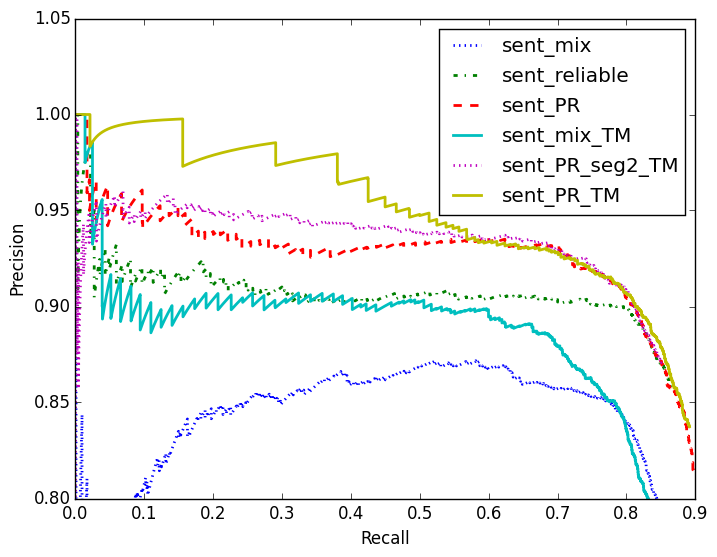
\includegraphics[width=0.9\linewidth]{figures/sent_time_exp_overall.png}
\caption{Sentence Level Results on TimeRE}
\label{fig: sent_luo}
\end{center}
\end{figure}

\subsection{Experimental Setup}

\paragraph{Hyperparameters} \red{can we put those parameters in a table?? especially those shared by the two settings.} \todo{ZW: Agree. These parameters should be given in a table!}
We experiment our sentence level model on \TimeRE. We use 100-dimensional word embedding pre-trained using GloVe \cite{pennington2014glove} on Wikipedia and Gigaword, and 20-dimensional vector for distance embedding. The convolution window is 3 and the number of convolution kernels is 200. The size of the full connection layer is also 200. As for training, we use stochastic gradient descend (SGD) with batch size 20, learning rate 0.1. We also use dropout with probability 0.5 upon the sentence embedding. Each data subset is added after 15 epochs since the precious one is added. The trace regularization parameters for three subsets are $\beta_1=-0.01$, $\beta_2=0.01$ and $\beta_3=0.1$ respectively from the reliable one to the most unreliable one (the ratio of $\beta_3$ and $\beta_2$ is fixed to 10 or 5 during hyper-parameter tuning).


The parameters of the bag level model is almost the same as the sentence level model on TimeRE data, except that the learning rate is 0.01. As for the \EntityRE data, the word embedding is of dimension 50 and is pre-trained on the NYT corpus using word2vec\footnote{\url{ https://code.google.com/p/word2vec/}}. The convolution window is 3 and the number of convolution kernels is 256, distance embedding size is 5, batch size is 16 and learning rate is 0.01. For all the bag level models, the linear combination parameter $\alpha$ is 1 and trace regularization parameter $\beta$ is -0.1 at the start of training. We experiment with decay rate \{0.95, 0.9, 0.8\} and decay step \{3, 5, 8\}. We find that using decay rate 0.9 and decay step 5 performs best in most situations.

\paragraph{Evaluation Metrics}
We evaluate the relation extraction performances using precision-recall (\PR) curves, which is calculated according to the extraction results ranked decreasingly by confidence score.

\paragraph{Baseline Settings}
We evaluate our approach under two extraction settings, sentence level
(\texttt{sent\_}) and bag level (\texttt{bag\_}). In both settings, we
investigate models trained on all subsets mixed together (\texttt{\_mix}),
models trained on reliable data only (\texttt{\_reliable}), models trained
with transition matrix (\texttt{\_TM}), and models trained models trained
with the curriculum learning setting  (\texttt{\_CL}). In the bag level
experiments, we also study the effect of attention (\texttt{\_att}) and
average
(\texttt{\_avg}) aggregation methods.
\todo{ZW: This paragraph need to be polished.}

\begin{figure*}[htbp]
\centering
\subfigure[Attention Aggregation]{
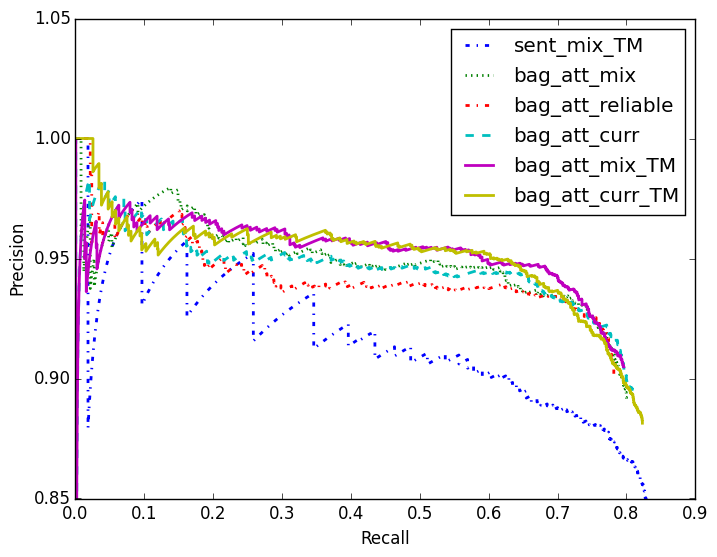
\includegraphics[width=0.45\linewidth]{figures/bag_att_exp_overall.png}
\label{fig: bag_att_luo}
}
\subfigure[Average Aggregation]{
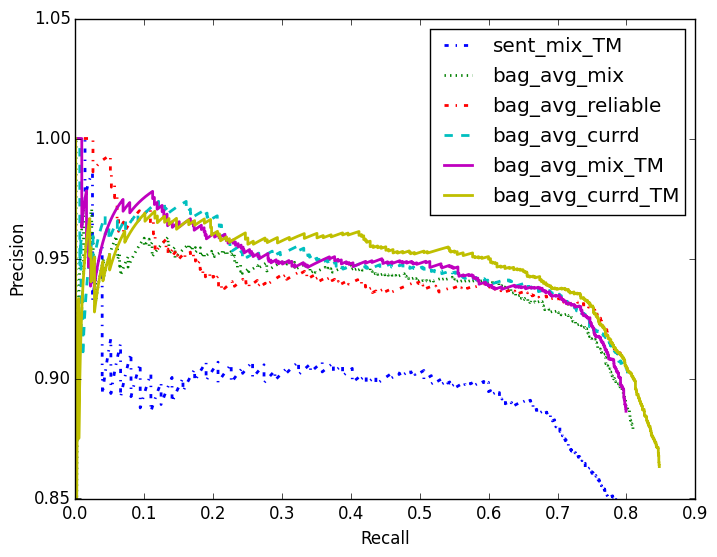
\includegraphics[width=0.45\linewidth]{figures/bag_avg_exp_overall.png}
\label{fig: bag_avg_luo}
}
\caption{Bag Level Results on TimeRE}
\label{fig: results_on_luo}
\end{figure*}

\subsection{Evaluation on \TimeRE}
\paragraph{Sentence Level Models}
The results of sentence level models on \TimeRE are shown in Figure \ref{fig:
sent_luo}. We can see that mixing all subsets together (\texttt{sent\_mix})
gives the worst result. The performance of this strategey is significantly
worse than using the reliable subset only (\texttt{sent\_reliable}). This
suggests the noisy nature of the training data obtained through \DS and
properly dealing with the noise is the key for \DS to be adopted at a wider
scale. When getting help from our transition matrix during training, the
model (\texttt{sent\_mix\_TM}) significantly improves (\texttt{sent\_mix}),
delivering the same level of performance as (\texttt{sent\_reliable}) in most
cases. This suggests that our transition matrix can help to mitigate the bad influence of noisy training instances.


Let us consider the scenario where the training is first performed on the
reliable subset first and then gradually moved to the space with less
reliable data. In this case, the curriculum learning based model
(\texttt{sent\_CL}) even  outperforms \emph{sent\_reliable} significantly,
indicating that the curriculum learning framework not only reduces the effect
of noise, but also helps the model learns from noisy data. When applying the
transition matrix into the curriculum learning framework using one reliable
subset and one less reliable one,   our model (\emph{sent\_CL\_seg2\_TM})
improves \emph{sent\_CL} by exploring the prior knowledge about data quality
and enable the transition matrix approach to control the noise in different
levels. \todo{ZW: Have no idea of what this sentence is talking about.} It is
not surprising that when we use more less reliable data, i.e., using all
three subsets, our model (\emph{sent\_CL\_TM}) significantly outperforms all
other models by a large margin\footnote{We will use all three subsets for all
\emph{\_CL\_TM} settings in the rest of the experiments.}. \todo{ZW: I
rephrase some of the sentences, but I still think this paragraph needs to be
written.}


\paragraph{Bag Level Models}
In this experiment, we first look at the performance of the bag level models with attention aggregation. The results are shown in Figure \ref{fig: bag_att_luo}.
Consider a comparatione between the  model trained on the reliable subset only (\texttt{bag\_att\_reliable}) and  the model trained on the mixed dataset (\texttt{bag\_att\_mix}).
In contrast to the sentence level cases, \texttt{bag\_att\_mix} outperforms \texttt{bag\_att\_reliable} by a large margin. This is due to the fact that  \texttt{bag\_att\_mix} has taken the noise within the bag into consideration through the attention aggregation mechanism, which can be seen as a denoising step within the bag.
This may also be the reason that when we introduce either our transition matrix approach \red{(\texttt{bag\_att\_TM})}  or curriculum learning framework (\texttt{bag\_att\_CL})   into the bad level model , the improvement compared to \texttt{bag\_att\_mix}  is not as significant as in the sentence level.
However, when we utilize our transition matrix approach to control the noise ate different levels within the curriculum learning paradigm (\texttt{bag\_att\_CL\_TM}), the performance gets further improved. This is especially in the high precision part compared to \texttt{bag\_att\_CL}.
We also note that the bag level's  \textit{at-least-one assumption} does not always hold, and there are still false negative and false positive problems. Therefore, we can see that using our transition matrix approach with  or without curriculum learning, i.e.,  \texttt{bag\_att\_TM}  and \texttt{bag\_att\_CL\_TM}), both improve the performance, and \texttt{bag\_att\_CL\_TM} performs slightly better.

%\paragraph{Bag Level Average Aggregation Models}
The results of the bag level models with average aggregation is shown in Figure \ref{fig: bag_avg_luo}. The relative ranking of various settings is similar to those with the attention aggregation. \red{why (\texttt{bag\_avg\_reliable}) performs so much better than all others in the very high precision stage ($recall<0.05$)?????????} One of the notable differences is that both \texttt{bag\_avg\_CL} and \texttt{bag\_avg\_TM} improve \texttt{bag\_avg\_mix} with larger margins compared to that in the attention aggregation setting. The reasons may be that the average aggregation mechanism is not as good as the attention aggregation one in terms of denoising ability, which leaves more space for our transition matrix approach or curriculum learning framework to improve.
\blue{Another prominent difference lies in the performance drop of \emph{bag\_avg\_CL\_TM} in the low-recall area ($recall<0.15$)., why???}
%However, since  denoising ability is not as good as attention aggregation, adding unreliable data gradually (\emph{bag\_avg\_currd}) improves the model performance here. We can also see that the transition matrix improves the average aggregation models more significantly than the attention aggregation models.
 %Note that due to the inferior denoising ability of average aggregation, the unhandled sentence level noise may further propagates to bag level, which gives the transition matrix more chance to help model the noise.

\begin{figure}[htbp]
\begin{center}
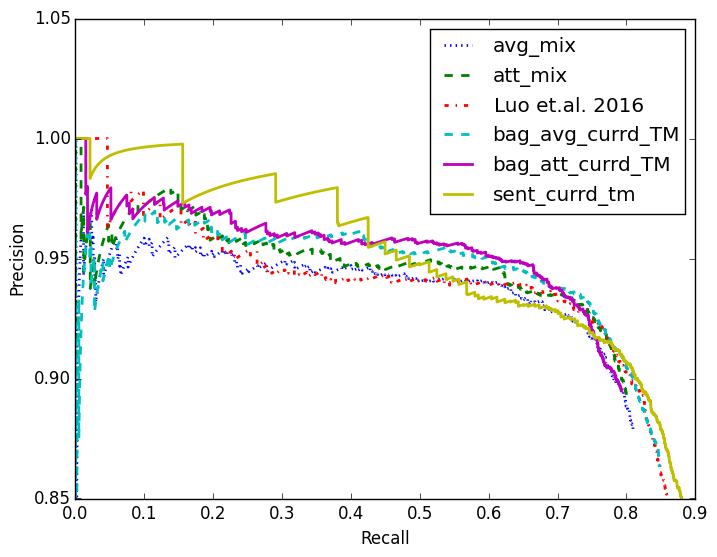
\includegraphics[width=0.9\linewidth]{figures/best_cmp_exp_overall.png}
\caption{Comparison on TimeRE}
\label{fig: cmp_luo}
\end{center}
\end{figure}

\paragraph{Compare to the-state-of-the-art} \red{should change to something else??? e.g., case study, or static TM }
The comparison of the best settings of each model family is shown in Figure \ref{fig: cmp_luo}. We can see that all of our transition matrix models outperform a state-the-art model presented in \cite{luo2016temporal}. With the help of transition matrix, although the basic version of average aggregation is not as good as attention aggregation, its transition matrix version is similar to the attention aggregation. Also note that although the sentence level models trained on mixed data do not perform very good, the sentence level model can use transition matrix to model the sentence level noise and thus performs best in all these models. Recall that the transition matrix can model the noise rather than just reduce the influence of noisy sentences as in bag level models, the sentence level model actually has the ability to make use of the noisy data. This shows that sentence level noise is more significant than the bag level noise in relation extraction, and modeling noise works better than just trying to reducing the influence of noise.


\begin{figure}[t!]
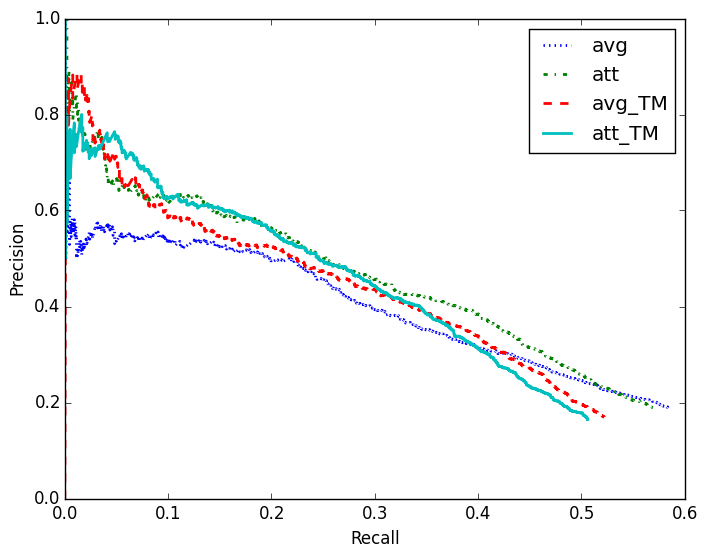
\includegraphics[width=0.9\linewidth]{figures/re_att_avg_cmp_exp.png}
\caption{Results on Dataset of Riedel et.al.}
\label{fig: Riedel_res}
\end{figure}

\subsection{Performance on \EntityRE}
We also conduct experiments on the \EntityRE dataset, where we can evaluate our bag level models only. \todo{ZW: Why bag-level models only? We need a an answer!}
We  implemented the average aggregation method (\texttt{avg}), and the attention aggregation method (\texttt{att}) proposed by \cite{lin2016neural} as well as their corresponding transition matrix versions (\texttt{avg\_TM} and \texttt{att\_TM}). As we can see in Figure \ref{fig: Riedel_res},  due to the inferior denoising ability of the average aggregation component, \texttt{avg} performs worst among all those models. %Similar to the trends on the TimeRE data, when
\red{what should we say about this figure????}
When we inject our transition matrix approach into both \emph{avg} and \emph{att}, the resulting two  models, both of which can  clearly outperform their basic extraction models.
%
%since the unhandled sentence level noise propagates to the bag level, which makes the bag level noise become more severe, the transition matrix has more chance to model the noise. Therefore, the \emph{avg\_TM} model clearly outperforms the \emph{avg} model.
Again, because the attention aggregation model , this model already has good ability in reducing the impact of sentence level noise. Since the bag level noise is less significant than the sentence level noise, the improvement of our transition matrix model is limited, which only improves the model on the low recall part.
%Note that the low recall part corresponds to high precision, which is more useful than the rest of the extraction results in practice. Therefore, our transition matrix method is also useful in this situation.

\iffalse
\begin{figure*}[htbp]
\centering
\subfigure[Overall PR Curves]{
\includegraphics[width=0.475\linewidth]{reg_exp_overall.png}
\label{fig: reg_overall_pr_curve}
}
\subfigure[Small Relation PR Curves]{
\includegraphics[width=0.475\linewidth]{reg_exp_small.png}
\label{fig: reg_small_rel_pr_curve}
}
\caption{Imapct of Regularization Weights}
\label{fig: reg_PR_curve}
\end{figure*}
\fi

\paragraph{Summary}
\todo{ZW: This section is incredibly complex. I suggest to have a summary section to highlight the take away messages.}
